%{{{
\documentclass[
12pt,
a4paper,
portuges,
draft
]{report}

\usepackage[
top=3cm,
left=3cm,
bottom=2cm,
right=2cm
% inner=1.5in, % The inner margin (beside binding)
% outer=1in, % The outer margin (opposite binding)
% headheight=20pt, % Header height
% headsep=.25in, % Header separation
% includehead,
% includefoot
]{geometry}

\usepackage[portuges]{babel}
%times new roman package
\usepackage[utf8]{inputenc}
\usepackage[T1]{fontenc}
\usepackage{mathptmx}
\usepackage{titling}
\usepackage{fancyhdr}
\usepackage{anyfontsize}
\usepackage{indentfirst}
\usepackage{csquotes}

\pagestyle{myheadings}
%ovewrite plain to my headings style
\makeatletter
  \let\ps@plain\ps@myheadings
\makeatother

\usepackage{titlesec}
\usepackage[final]{graphicx}
\graphicspath{ {asset/} }
%sort by alphabetic label, name, year, volume, title 
\usepackage[citestyle=authoryear,backend=bibtex,sorting=anyvt]{biblatex}
\addbibresource{tcc.bib}
\addto\captionsportuges{
	\renewcommand{\contentsname}{\hspace*{\fill} SUMÁRIO\hspace*{\fill}}
    \renewcommand{\listfigurename}{\hspace*{\fill} LISTA DE FIGURAS\hspace*{\fill}}
    \renewcommand{\chaptername}{}
    \renewcommand{\figurename}{Fig.}
}

\usepackage{setspace}

\titleformat{\chapter}{\normalfont\fontsize{14}{17}\bfseries}{\thechapter}{1em}{}
\titleformat{\section}{\normalfont\fontsize{12}{15}\bfseries}{\thesection}{1em}{}
\titleformat{\subsection}{\normalfont\fontsize{12}{15}\bfseries}{\thesubsection}{1em}{}
\titleformat{\subsubsection}{\normalfont\fontsize{12}{15}\bfseries}{\thesubsubsection}{1em}{}

\renewenvironment{quote}
               {\list{}{\rightmargin\leftmargin}%
                \item\relax\fontsize{10}{12}}
               {\endlist}

\usepackage{titletoc}
\usepackage{tocloft}
\setlength{\cftchapindent}{0cm}
\setlength{\cftsecindent}{0cm}
\setlength{\cftsubsecindent}{0cm}
\setlength{\cftsubsubsecindent}{0cm}
\dottedcontents{chapter}[1.5em]{}{1.3em}{.6em}


\renewcommand\cfttoctitlefont{\normalfont\fontsize{14}{17}}
\renewcommand\cftloftitlefont{\normalfont\fontsize{14}{17}}
%\renewcommand\cftfigfont{\normalfont\fontsize{10}{12}}
%\renewcommand\cftfigpagefont{\normalfont\fontsize{10}{12}}


\DefineBibliographyStrings{portuguese}{%
%  backrefpage = {<newtext>},
%  backrefpages= {<newtext>},
  urlseen = {Disponível em},
  url = {Disponível em}
}
\DeclareFieldFormat{url}{\bibstring{url}\space\url{#1}}
\DeclareFieldFormat{urlseen}{\bibstring{urlseen}\space\url{#1}}

%{{{ VARIABLES
\title{\uppercase{Limitações do HTML5 \\ no desenvolvimento de jogos multiplataforma}}
\author{\uppercase{Jean Carlo Machado}}
\newcommand{\supervisor}{Mr. Rafael Jaques}
\newcommand{\university}{\uppercase{Instituto Federal de Educação, Ciência \\ e Tecnologia do Rio Grande do Sul \\ Campus Bento Gonçalves}}
\newcommand{\locale}{Bento Gonçalves, Dezembro 2015}
\newcommand{\website}{http://jeancarlomachado.com.br}
%}}}

\begin{document}
\pagenumbering{gobble}
%}}}

%{{{Title Page

\begin{titlepage}
    \begin{center}
        {\fontsize{14}{18}\selectfont \university}
        \vfill
        {\fontsize{16}{19}\selectfont \thetitle }
        \vfill
        {\fontsize{12}{15}\selectfont \theauthor}
        \vfill
        {\locale}
    \end{center}
\end{titlepage}

%}}}

%{{{Folha de rosto

\begin{titlepage}
    \begin{center}
        {\fontsize{14}{18}\selectfont \theauthor}
        \vfill
        {\fontsize{16}{19}\selectfont \thetitle }
        \vfill
        \hfill
        \parbox[s]{8cm}{
        \singlespacing
            Monografia apresentada junto ao Curso
        de Tecnologia em Análise e Desenvolvimento de Sistemas no
    Instituto Federal de Educação, Ciência e Tecnologia do Rio
Grande do Sul - Campus Bento Gonçalves, como requisito parcial à
obtenção do título de Tecnólogo em Análise e Desenvolvimento de Sistemas.
        \\
        Orientador: Mr. Rafael Jaques
        }
        \vfill
        {\bfseries \locale}
    \end{center}
\end{titlepage}

%}}}
\onehalfspacing
%{{{ Resumo
\renewcommand{\abstractname}{\Large\bfseries RESUMO}
\begin{abstract}
{ LLorem ipsum dolor sit amet, consectetur adipiscing elit, sed do eiusmod tempor incididunt ut labore et dolore magna aliqua. Ut enim ad minim veniam, quis nostrud exercitation ullamco laboris nisi ut aliquip ex ea commodo consequat. Duis aute irure dolor in reprehenderit in voluptate velit esse cillum dolore eu fugiat nulla pariatur. Excepteur sint occaecat cupidatat non proident, sunt in culpa qui officia deserunt mollit anim id est laborum.

orem ipsum dolor sit amet, consectetur adipiscing elit, sed do eiusmod tempor incididunt ut labore et dolore magna aliqua. Ut enim ad minim veniam, quis nostrud exercitation ullamco laboris nisi ut aliquip ex ea commodo consequat. Duis aute irure dolor in reprehenderit in voluptate velit esse cillum dolore eu fugiat nulla pariatur. Excepteur sint occaecat cupidatat non proident, sunt in culpa qui officia deserunt mollit anim id est laborum.
}

{\bfseries Palavras-chave:} HTML5, Limitações, Jogos,
Multiplataforma
\end{abstract}


\renewcommand{\abstractname}{\Large\bfseries ABSTRACT}
\begin{abstract}
{ LLorem ipsum dolor sit amet, consectetur adipiscing elit, sed do eiusmod tempor incididunt ut labore et dolore magna aliqua. Ut enim ad minim veniam, quis nostrud exercitation ullamco laboris nisi ut aliquip ex ea commodo consequat. Duis aute irure dolor in reprehenderit in voluptate velit esse cillum dolore eu fugiat nulla pariatur. Excepteur sint occaecat cupidatat non proident, sunt in culpa qui officia deserunt mollit anim id est laborum.

orem ipsum dolor sit amet, consectetur adipiscing elit, sed do eiusmod tempor incididunt ut labore et dolore magna aliqua. Ut enim ad minim veniam, quis nostrud exercitation ullamco laboris nisi ut aliquip ex ea commodo consequat. Duis aute irure dolor in reprehenderit in voluptate velit esse cillum dolore eu fugiat nulla pariatur. Excepteur sint occaecat cupidatat non proident, sunt in culpa qui officia deserunt mollit anim id est laborum.
}

{\bfseries Palavras-chave:} HTML5, Limitações, Jogos,
Multiplataforma
\end{abstract}

%}}}

{\listoffigures}
\clearpage
{\tableofcontents}
%\listoftables
\chapter{CONTEXTUALIZAÇÃO}%{{{
\pagenumbering{arabic}
%\setcounter{page}{1} 

\section{JOGOS}

\subsection{BENEFÍCIOS}
Desenvolvedores de jogos web podem rapidamente satisfazer as
necessidades de seus jogadores, mantendo-os leais a tecnologia HTML5
\autocite{developingEffect}.

A maioria dos desenvolvedores demonstra interesse para o HTML5. (referenciar)

O tempo de desenvolvimento de uma aplicação em HTML5 é 67\% menor (referenciar)
que aplicações nativas. Isso mostra o custo efetivo de aplicações baseadas em HTML5. 

A real vantagem de aplicações em HTML5 é o suporte
horizontal entre as plataformas - que é a maior razão por trás do
custo efetivo. (HASAN et al, 2012)

\subsection{O MERCADO}

A maior dificuldade em capturar uma base de usuários é que o mercado
de dispositivos móveis é muito fragmentado e não existe uma única
plataforma popular. (HASAN, 2012)

Segundo \cite{HTML5CrossPlatformGameDevelopment}: 80\% do tempo total gasto usando dispositivos móveis é para a utilização de aplicativos, e 32\% é para jogar vídeo games.


\subsection{JOGOS E MULTIPLATAFORMA}

\subsection{HTML E MULTIPLATAFORMA}

\subsection{LIMITAÇÕES DE JOGOS MULTIPLATAFORMA COM HTML5}

Funcionalidades foram disponibilizadas de diversas fontes e não foram
construídas de forma consistente com as demais. Além
disso, devida a única característica da Web, erros de implementação
se tornam frequentes, e muitas vezes se tornam o padrão, pois outras
funcionalidades dependem destas primeiras antes que elas estejam
estáveis. (W3C manual)

Enquanto o HTML é desenvolvido muitas das funcionalidades
disponibilizadas são testadas em apenas um pequeno conjunto de
navegadores para um pequeno conjunto de versões (referência 2). Isso
acarreta em suporte inconsistente. A forma mais segura de garantir
suporte é testando em todas as versões alvo, todavia essa solução
não é prática. (ref. 2)

Os desenvolvedores de navegadores podem interpretar/implementar
as especificações erroneamente aumentando os problemas de
compatibilidade.


\section{ESTE TRABALHO}

Este projeto propõe analisar as limitações do HTML5 quanto relativo
a construção de jogos multiplataforma. Através de revisão
bibliográfica e da criação de um protótipo de jogo multiplataforma.

Um tratado completo sobre o assunto requiriria um comparativo entre
jogos desenvolvidos nativamente e jogos em HTML5.

\subsection{O JOGO}

Para a análise prática das limitações foi escolhido um jogo de
matemática simples. Consistindo na geração de equações com um
candidato de resposta. Cabe ao usuário informar se o resultado apontado
pelo jogo está correto ou não.

Porquê escolhi esse tipo de jogo?
%}}}

\chapter{PROBLEMA}
%{{{

A carência de definições concretas sobre a viabilidade da atual
versão do HTML5 - aplicado ao desenvolvimento de jogos. O senso comum, 
acostumado com soluções nativas, acabam por monopolizar à construção de jogos nativos.

Os custos introduzidos no ciclo vida de um jogo, para diversas
plataformas, é muito alto para ser considerado trivial. Cerca de 65%
mais altos (segundo trabalho 2)
%}}}

\section{OBJETIVOS}
%{{{

\subsection{OBJETIVO GERAL}
%{{{

Identificar possíveis limitações no processo de desenvolvimento
de jogos multiplataforma oriundas do atual estado de definição e
implementação do HTML5.

Não é objetivo deste trabalho demonstrar os pontos fortes do HTML5,
apenas suas limitações. Também não é objetivo deste trabalho
comparar o HTML com outras tecnologias de desenvolvimento de jogos, c
omo Flash Player, Silverlight ou alternativas Desktop.
%}}}

\subsection{OBJETIVOS ESPECÍFICOS}

Estudar as limitações de desenvolvimento de jogos nas plataformas
Android e navegadores Desktop Google Chrome
e Firefox. Os navegadores foram testados em suas últimas versões.

Optamos por Android, e não IOS, pois o primeiro contém
a vasta maioria do mercado de dispositivos inteligentes, e por termos
maior experiência na já mencionada plataforma.

Construir um protótipo que colabore para a fundamentação prática do assunto.

Pretende-se também estudar os seguintes tópicos do desenvolvimento de
jogos, relativos ao HTML5:

\cite{browserGamesTechnologyAndFuture} cita que video, audio, drag
and drop, funcionalidades de gráficos e armazenamento off-line são
aspectos importantes do HTML5 para o desenvolvimento de jogos.

Com base nos estudos efetuados e na experiência adquirida elencamos os
seguintes itens que serão abordados neste estudo.

\begin{itemize}
\item Performance
\item Depuração
\item Diferenças em tamanho de tela
\item Canvas
\item Empacotadores HTML5
\item Eventos de entrada
\item Vibração
\item Acelerômetro
\item Armazenamento
\item Disponibilização de assets (controle de tamanhos, cache, etc)
\item Aplicações offline
\item CSS media queries
\end{itemize}

Elaborar uma lista de limitações e correlacionar os dados de acordo
com as plataformas.

%}}}

\chapter{JUSTIFICATIVA}
%{{{

Tendo em vista que este trabalho busca mapear possíveis problemas
do desenvolvimento multiplataforma em HTML ele serve para apoiar
e justificar decisões relativas ao desenvolvimento de jogos
multiplataforma.

Tem potencial apontar os pontos chave que necessitam
de melhorias no HTML, consequentemente colaborando para a
melhoria da própria especificação.
Estimular e avançar o estudo da implementação da Open Web;

A opinião comum tende para soluções nativas em detrimento do
desenvolvimento de jogos, este trabalho pretende desafiar esta
concepção. %REFERENCIAR

Muitos desenvolvedores estão familiarizados
com as tecnologias da WEB ou apontam interesse na tecnologia.


%}}}

\chapter{REVISÃO BIBLIOGRÁFICA}
%{{{

\section{JOGOS}
%{{{
Segundo \autocite{indieGamesLemes} jogo digital constitui-se em uma
atividade lúdica composta por uma série de ações e decisões,
limitada por regras e pelo universo do game, que resultam em uma
condição final.

Video games melhoram as funções cognitivas, melhoram as capacidades criativas, e
motivam uma visão positiva diante a falha \autocite{gamebenefits}.

%Mencionar algum jogo (como WOW) e como ele faz para prender a atenção dos usuários. Candy Crush saga

\subsection{GÊNEROS}

Uma classificação de jogos em gêneros é uma tarefa complexa. Segundo \autocite{gamebenefits}:

\begin{quote}
Pela diversidade  em itens e gêneros e a vasta quantidade de dimensões que os video games se encontram, uma taxonomia dos jogos contemporâneos é extremamente difícil de desenvolver (muitos já tentaram) .
\end{quote}


Não obstante alguns padrões são discerníveis quanto aos jogos da web.


Os primeiros jogos eram limitados a tecnologias presentes, um gênero de que se desenvolveu bem foram os jogos
de estratégia como o Travian.

Com as novas possibilidades do tecnológicas novas possibilidades e gêneros de jogos podem ser explorados na web.

\subsection{MECÂNICA}

A mecânica é composta pelas regras do jogo. Quais as ações
disponíveis aos usuários, é fortemente influenciada pela categoria do
jogo em questão.

\section{JOGOS MULTIPLATAFORMA}

Jogos em plataformas móveis trazem um novo conjunto de desafios para
produtores de jogos. Um destes desafios é fornecer feedback suficiente
para o jogador pois o dispositivo é limitado em proporções, som, tela
etc.

A interface tem que ser o mais intuitiva o possível. No caso de
dispositivos móveis, quanto menos gestos necessários melhor. Tornar
previsível causa e efeito é uma boa característica para os jogos.
Os desenvolvedores tem que evitar fazer o jogo para eles mesmos.
E pela falta de crítica os designs tendem a ser ruins. Afinal o
que os jogadores querem? LEMES (2009, pg XX) aponta alguns fatores procurados
pelos usuários de jogos: Desafio, socializar, experiência solitária,
respeito e fantasia.

Designers de jogos tem as seguintes possibilidades arquiteturais
quando em face de desenvolver um novo jogo: Criar um jogo web,
um jogo híbrido, ou nativo. As opções serão descritas abaixo.

\subsection{JOGOS WEB}

Um jogo web é um jogo que utiliza o HTML e
ferramentas correlacionadas para sua construção. Este tipo de jogo
é o que será abordado neste trabalho.

Entre seus pontos positivos pode-se listar:

\begin{itemize}
\item Necessitam de uma única base de código e pode rodar em todas as
plataformas;
\item Contém a mais vasta gama de desenvolvedores e muitos
interessados em aprendê-la;
\item Seus custos são inferiores, aos do desenvolvimento nativo devido a 
inexistência de duplicação da base de código;
\item  Não requerem instalação ou atualizações manuais
\item  Sua distribuição é superior ao estilo convencional de aplicações desktop\autocite{browserGamesTechnologyAndFuture}
\end{itemize}

Os pontos negativos dessa abordagem são o principal foco deste trabalho.

Mas a um nível macroscópico podemos citar:
\begin{itemize}
\item Programas que rodam na web são geralmente mais lentos que os
nativos;
\item Por falta de especificação ou incompletude de implementação.
\item Nem todos os recursos disponíveis através das SDK's nativas estão presentes através do HTML5.
\end{itemize}

Além dos jogos web, há a possibilidade de criar jogos híbridos e nativos.

\subsection{JOGOS HÍBRIDOS}

Jogos híbridos são jogos geralmente desenvolvidos com tecnologias da
web que rodam nativamente.

\subsection{DESENVOLVIMENTO DE JOGOS NATIVOS}

Pontos fortes:
\begin{itemize}
\item Habilita a melhor experiência de usuário pois permite utilizar ao
máximo os recursos e funcionalidades dos dispositivos.
\end{itemize}

Pontos fracos:
\begin{itemize}
\item Porém, devido a cada plataforma conter seu próprio sistema operacional,
com seus próprios *SDK's* totalmente incompatíveis, os desenvolvedores são
forçados a desenvolver uma versão do jogo para cada plataforma alvo.
\item Requer mais pessoas, e maior custo com possivelmente parte do mercado não atendido de qualquer forma.
\end{itemize}

%}}}

\section{WEB}
%{{{

\subsection{OPEN WEB}

A OWP (\textit{Open Web Platform}), uma coleção de tecnologias livres,
amplamente utilizadas e padronizadas.
Quando uma tecnologia se torna amplamente popular, através da
adoção de grandes empresas e desenvolvedores ela se torna candidata a
adoção pela OWP.

Mais do que um conjunto de tecnologias Open Web, é um conjunto de
filosofias as quais a web se baseia.

Neste conjunto inclui-se:

\begin{itemize}
\item Descentralização;
\item Transparência;
\item Relevância;
\item Imparcialidade;
\item Consenso;
\item Disponibilidade;
\item Manutibilidade;
\end{itemize}

A tecnologia chave que inaugurou e alavancou este processo é o HTML.
%}}}

\section{HTML}
%{{{

HTML (\textit{Hyper Text Markup Language}) é uma linguagem de
marcação que define a estrutura semântica do conteúdo das páginas
da web. Criada por Tim Berners Lee em 1989 no CERN. HTML é a tecnologia
base para a criação de páginas web e aplicativos online. A parte
denominada: "Hipertexto", refere-se a links que conectam páginas umas
as outras, fazendo a Web como conhecemos hoje
\autocite{mdn2015}.

HTML foi especificado baseando-se no padrão SGML (\textit{Standard Generalized
Markup Language}).

Alguns benefícios do SGML são:
\begin{itemize}
    \item Documentos declaram estrutura, diferentemente de aparência
- possibilitando otimizações nos ambientes de uso (tamanho de tela,
etc);
    \item São portáveis devido a definição de tipo de documento
(\textit{document type declaration});
\end{itemize}

Apesar de o SGML negar a definição de aparência, os criadores de
navegadores constantemente introduziam elementos de apresentação como o
piscar, itálico, e negrito, que eventualmente acabavam por serem inclusos
na especificação. Foi somente nas últimas versões que elementos de
apresentação voltaram a ser proibidos reforçando as propostas chave
HTML como uma linguagem de conteúdo semântico, incentivando a
utilização de outras tecnologias, como o CSS, para responder as demandas de
apresentação.

Além do HTML, existe o XHTML, que é uma iniciativa de utilização
de XML nas páginas da web. O XML é um padrão mais rigoroso que SGML
e resulta em páginas válidas, que podem ser mais facilmente interpretadas por
outras tecnologias, como sistemas de terceiros, etc.

Para transformar o HTML em algo visível os navegadores, através
de motores de renderização, decodificam um documento HTML
em objetos em memória. Este processo é denominado tokenização.

Diferentemente do XHTML, HTML não pode ser decodificado através de
tokenização tradicional. Deve-se ao HTML ser amigável ao programador,
aceitando erros de sintaxe, dependente de contexto, buscando entregar a
melhor aproximação possível. Esta característica deu origem a uma
especificação para renderizar HTML (\textit{HTML parser}).

A última versão do HTML é o HTML5, iniciado pela WHATWG
e posteriormente desenvolvido em conjunto com a W3C.
Seu rascunho foi proposto em 2008 e ratificado em 2014.
Após 2011, a última chamada de revisão do HTML5,
a WHATWG decidiu renomear o HTML5 para HTML
\autocite{htmlIsTheNewHtml5}. Não obstante, o termo HTML5
permanece em utilização pela W3C.

Além da nomenclatura, exitem pequenas diferenças especificações da W3C e WHATWG. A
W3C vê a especificação do HTML5 como algo fechado, inclusive já
iniciou o desenvolvimento do HTML 5.1. Já a WHATWG vê o HTML5 como uma
especificação viva. A postura da W3C tende a criar uma especificação
mais estável, já a da W3C reflete mais a realidade dos navegadores,
que nunca implementam uma versão completamente. A Mozilla utiliza a
especificação da WHATWG no desenvolvimento do Firefox e recomenda a
da W3C para coisas que requeiram maior estabilidade. Neste trabalho
optamos pela nomenclatura da WHATWG, utilizamos o termo HTML em
detrimento a HTML5, sempre que semanticamente viável.

Antes do HTML5 várias versões foram propostas, algumas radicais
em seus preceitos. O XHTML 2.0, por exemplo, quebrava com toda
a compatibilidade das versões anteriores e acabou por sendo descontinuado.
Outrossim, a maioria das versões HTML de grande sucesso foram versões de
retrospectiva (\textit{"retro-specs"}). Versões que não tentavam
idealizar a linguagem, buscando alinhar-se com os requerimentos do
mercado \autocite{diveIntohtml}.

Uma página HTML consiste em elementos que podem ter seu comportamento
alterado através de atributos. Um elemento é o abrir fechar de
uma tag e todo o conteúdo que dentro dele reside \autocite[pp.
10--11]{htmlAndCssDucket}. Na figura \ref{fig:htmlSample} o elemento
meta tem um atributo \textit{charset}. Note também que os elementos
estão aninhados em forma de grafo, esta estrutura também é conhecida como DOM.


\subsection{DOM}
%{{{

O modelo de documento de objetos (\textit{Document Object Model}) é a representação
em memória de uma árvore de elementos HTML. Esta representação é definida por
um conjunto de padrões que torna interoperável a manipulação de elementos através de
JavaScript.

A primeira versão do DOM, (DOM Legacy) foi parcialmente especificada no HTML4.
O DOM é também uma forma de manter estado em páginas HTML.
Os navegadores contam com as engines de layout para parsear HTML em DOM.
A atual versão do DOM é a versão 3

%}}}


\begin{figure}
\centering
\begin{verbatim}
<!DOCTYPE HTML>
<html lang="en-US">
<head>
	<meta charset="UTF-8">
	<title></title>
</head>
<body>
    <video>
        <span>Seu navegador não suporta vídeo</span>
    </video>
</body>
</html>
\end{verbatim}
\caption{Exemplo de documento HTML5}
\label{fig:htmlSample}
\end{figure}

Na sua versão inicial, o HTML contava com 18 elementos;
atualmente existem mais de cem \autocite{diveIntohtml}.
Não obstante, foi no HTML5 que a maior parte dos elementos
que viabilizam a construção de jogos foram adicionados.

Visto que nenhum navegador implementa a especificação completamente,
cabe ao desenvolvedor detectar os navegadores que não comportam as
necessidades tecnológicas. Ao deparar-se com uma funcionalidade
faltante o desenvovedor tem duas possiblidades polyfills ou notificar o usuário.

Polyfills são recursos que simulam uma funcionalidade não disponível para
os navegadores que não suportam determinada especificação. %exemplificar

Um dos objetivos do HTML é manter a retrocompatiblidade,
o HTML atinge isso ignorando os elementos que não conhece, tratando apenas
seu vocabuliário. Esse mecanismo permite que os desenvedores incluam
marcação de reserva dentro dos elementos que podem ser não suportados.
O elemento span na \ref{fig:htmlSample} só aparecerá para o usuário caso seu
navegador não suporte a tag vídeo.

Uma boa referência de recursos suportados pelos navegadores é o site
http://caniuse.com/. A biblioteca Modernizr é uma boa ferramenta para
detectar suporte a recursos HTML nos navegadores.

Além da convencional linguagem de marcação; HTML5 ou "HTML5 e amigos"
é muitas vezes interpretado como um conceito guarda chuva para designar
as tecnologias da web HTML, CSS3 e JavaScript.

\begin{figure}
    \centering
    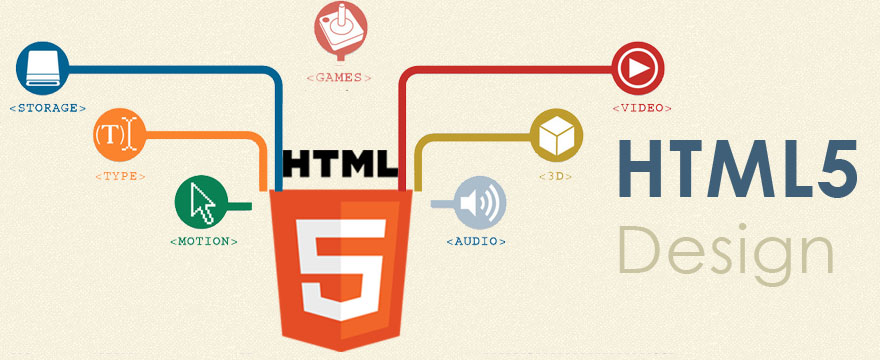
\includegraphics[width=0.8\textwidth,natwidth=610,natheight=642]{html5.jpg}
	\caption{Suite HTML5}
\end{figure}
%}}}


\section{CSS}
%{{{

CSS (\textit{Cascading Style Sheets}) é uma linguagem de folhas de
estilo, criada por Håkon Wium Lie em 1994, com intuito de definir a
apresentação de páginas HTML. O termo Cascading refere-se ao fato de
regras serem herdadas pelos filhos de um elemento, eliminando
grande parcela de duplicação de regras.

Antes do CSS a estilização das páginas era inclusa dentro do HTML. Isso era
negativo pois forçava que mudanças tivessem que ser replicadas em
todas suas ocorrências, e não permitia apresentações diferenciadas
para diferentes tipos de dispositivos. Com CSS também é possível o
usuário declarar suas folhas de estilo e alterar a visualização das páginas
que está vendo, um recurso importante para acessibilidade.

Segundo \cite[pp. 23--24]{CascadingStyleSheets}:
\begin{quote}
CSS possibilita a ligação tardia (\textit{late biding}) com páginas HTML. Essa característica
é atrativa para os publicadores por dois motivos. Primeiramente pois
permite o mesmo estilo em várias publicações, segundo pois os
publicadores podem focar-se no conteúdo.
\end{quote}


CSS é formado por um conjunto de regras, que são agrupadas
por seletores em blocos de declaração. Os elementos selecionados são
denominados o assunto do seletor \autocite{cssSelectors}. Seletores tem
o intuito de definir quais partes do documento HTML serão afetadas por
determinado bloco de declaração.

Sua última versão, o CSS3, introduziu várias funcionalidades
relevantes para jogos, como \textit{media-queries}: possibilitam regras para
tamanhos de tela, transformações 3D e animações.

O CSS é dividido em módulos, contendo aproximadamente 50 deles, cada
qual evoluindo separadamente.

Os navegadores interpretam CSS através da tag \textit{style}.

Muitos navegadores também suportam aceleração de GPU (Unidade de
processamento gráfico) para elementos que tenham transformações 3D.

Flow de documento, ordem e posição em que os elementos tem que
aparecer na página. Modelo de caixa o que encapsula o conteúdo em um
elementos.

%CSS has various levels and profiles. Each level of CSS builds upon the last, typically adding new features and typically denoted as CSS 1, CSS 2, CSS 3, and CSS 4. Profiles are typically a subset of one or more levels of CSS built for a particular device or user interface. Currently there are profiles for mobile devices, printers, and television sets. Profiles should not be confused with media types, which were added in CSS 2.%

%colocar uma imagem dos níveis do CSS

\subsection{Media Queries}

-falar de tamanhos absolutos vs relativos
sobre unidades em pixel, relativas e un.

Unidades vw e vh para tamanho do viewport



%falar do suporte a variáveis do CSS
\subsection{Transições}

É uma forma de adicionar animações de um estado para outro, em uma página web.

\subsection{Desabilitando elementos do navegador}
-overscroll
-addressbar
-touch-callout
-user select

%}}}

\section{JAVASCRIPT}
%{{{

EMACScript, melhor conhecido como JavaScript, criada por Brendan Eich
em 1992, é a linguagem da Web. Devido a tremenda popularidade entre
comunidade de desenvolvedores a linguagem foi abraçada pela W3C e
atualmente é um dos componentes da *Open Web Platform*.

As definições da linguagem são descritas na especificação ECMA-262.
Esta possibilitou o desenvolvimento de outras implementações além da
original - *SpiderMonkey* - como o Rhino, V8 e TraceMonkey; bem como
outras linguagens similares como JScript da Microsoft e o ActionScript
da Adobe.

JavaScript é uma linguagem de script. Segundo a Ecma Internacional
2012:

\begin{quote}
Uma linguagem de script é uma linguagem de programação que é
usada para manipular e automatizar os recursos presentes em um dado
sistema. Nesses sistemas funcionalidades já estão disponíveis
através de uma interface de usuário, uma linguagem de script é
um mecanismo para expor essas funcionalidades para um programa
protocolado.
\end{quote}

A intenção original era utilizar o JavaScript para dar suporte aos já
bem estabelecidos recursos do HTML, como para validação, alteração
de estado de elementos, etc. Em outras palavras, a utilização do
JavaScript era opcional e as páginas da web deveriam continuar
operantes sem a presença da linguagem.

Com a construção de projetos Web cada vez mais complexos,
as responsabilidades delegadas ao JavaScript aumentaram a ponto que a
grande maioria dos sistemas web não funcionarem sem ele. Não obstante,
JavaScript não evoluiu ao passo da demanda e muitas vezes carece de
definições expressivas, completude teórica, e outras características
de linguagens de programação mais bem estabelecidas, como o C++ ou
Java (Barnett, 2013). A nova versão do JavaScript, o JavaScript 6, é
um esforço nessa direção. JavaScript 6 ou *EMACScript Harmonia*,
contempla vários conceitos de orientação a objetos como classes,
interfaces, herança, tipos, etc.

Estes esforços de padronização muitas vezes não são rápidos
o suficiente para produtores de software web, demora-se muito até
obter-se um consenso sobre quais as funcionalidades desejadas em
determinada versão e seus detalhes de implementação. Outrossim, uma
vez definidas as especificações, é necessário que os distribuidores
do JavaScript implementem o especificado.

Alternativamente, existe uma vasta gama de conversores de código -
*transpilers* - para JavaScript; possibilitando programar em linguagens
formais e posteriormente gerar código JavaScript. Não obstante,
essa alternativa tem seus pontos fracos, necessita-se de mais tempo
de depuração , visto que o JavaScript gerado não é conhecido
pelo desenvolvedor, e provavelmente o código gerado não será tão
otimizado, nem utilizará os recursos mais recentes do JavaScript.

Mesmo com suas fraquezas amplamente conhecidas, JavaScript está
presente em praticamente todo navegador atual. Sendo uma espécie de
denominador comum entre as plataformas. Essa onipresença torna-o
integrante vital no processo de desenvolvimento de jogos multiplataforma
em HTML5. Vários títulos renomeados já foram produzidos que fazem
extensivo uso de JavaScript, são exemplos: Candy Crush Saga, Angry
Birds, Dune II, etc.

Jogos Web são escritos na arquitetura cliente servidor, JavaScript pode
rodar em ambos estes contextos, para tanto, sua especificação não
define recursos de plataforma. Distribuidores do JavaScript complementam
a o JavaScript com recursos específicos para suas plataformas alvo.
Por exemplo, para servidores, define-se objetos de terminal, acesso a
arquivos e dispositivos, etc. No contexto de cliente, são definidos
objetos como janelas, frames, DOM, etc.

Para o navegador o código JavaScript geralmente é disposto no elemento
``script`` dentro de arquivos HTML. Quando os navegadores encontram esse
elemento eles fazem a requisição para o servidor e injetam o código
retornado no documento, e a não ser que especificado de outra forma,
iniciam sua execução.


\subsection{ASM.JS}
Asm.js é um subconjunto da sintaxe do JavaScript a qual permite grandes
aumentos de performance quando em comparação com JavaScript normal.
No contexto dos jogos performance é usualmente um recurso estimável,
asm.js consegue-o supra utilizando recursos que permitam otimizações
antes do tempo *ahead of time optimizations*. Entretanto, não é
trivial escrever código em asm.js e geralmente a geração de código
asm.js é feita através da transpilação de outras linhagens como C.

Muita da performance adicional em relação ao JavaScript é devido
a consistência de tipo e a não existência de um coletor de lixo
(memória é gerenciada manualmente através de um grande vetor). Esse
modelo simples desprovido de comportamento dinâmico, sem alocação
e desalocação de memória, apenas um bem definido conjunto de
operações de inteiros e flutuantes possibilita grade performance e
abre espaço para otimizações.


%}}}

\section{RENDERIZAÇÃO}

Renderização é parte fundamental de muitos jogos. As tecnologias atualmente existes são o SVG e Canvas.

\subsection{SVG}
%{{{
SVG (\textit{Gráficos de vetores escaláveis}), é uma linguagem baseada em XML para marcar vetores bidimensionais e mapa de bits \autocite{html5mostwanted}.


Entre os benefícios do SVG encontram-se:

\begin{itemize}
\item Não há diferença de qualidade em resoluções pois os vetores são escaláveis;
\item Suporta animações nativamente;
\item Conta com integração através da api do DOM. Tornando simples a integração com as outras tecnologias da web.
\end{itemize}

\begin{figure}
\centering
\begin{verbatim}

<svg height="100" width="100">
  <circle cx="50" cy="50" r="40" stroke="black" stroke-width="3"/>
  Sorry, your browser does not support inline SVG.
</svg>

\end{verbatim}
\caption{Círculo em SVG.}
\end{figure}
%}}}

\subsection{CANVAS}
%%{{{

A tag \textit{canvas} define uma camada de mapa de bits em documentos
HTML que pode ser usada para criar diagramas, gráficos e animações
2D. Em um documento HTML, Canvas é um retângulo onde pode-se usar
JavaScript para desenhar \autocite{diveIntohtml}. Foi criada pela Apple
em 2004 para renderizar elementos de interface no Webkit, logo foi
adotado por outros navegadores e se tornou um padrão. A API canvas
cresceu com o tempo, e algumas funcionalidades - como suporte a texto,
foram adicionadas tardiamente. E alguns navegadores lançaram antes
da especificação estar completa e hoje tem problema de suporte para
essas áreas \autocite{diveIntohtml}. Apesar de muitas vezes incompleto,
o canvas é suportado em todos os maiores navegadores à partir do
Internet Explorer 9.

Tem dois tamanhos, o tamanho do elemento e da superfície de
desenho. Quando o tamanho do elemento é maior do que o da superfície
de desenho do documento escala a superfície de desenho para preencher o
elemento, o que pode gerar resultados inesperados.

Apesar de ser largamente suportado nos navegadores atuais, canvas ainda
sofre de problemas de performance. Para navegadores antigos - abaixo do
Internet Explorer 9 - existe a biblioteca Explorer Canvas do Google, que
emula em JavaScript as funcionalidades do canvas. O FastCanvas é uma
iniciativa híbrida para Android que busca mitigar os problemas de
performance do Canvas com uma API nativa. Não obstante, o FastCanvas
não suporta a especificação do canvas completamente, não permite ser
integrado com outros elementos do DOM.

Algumas outras fraquezas do canvas são:
\begin{itemize}
\item{Não há suporte a animações}
\item{Não é possível alterar uma parte já desenhada a não ser sobrescrevendo ou pintando o canvas novamente}
\item{Por ser um vetor de pixeis não existe possibilidade de utilização do DOM nem seus eventos, limitado muito a iteratividade}
\end{itemize}

O canvas até aqui descrito trata-se de sua forma, ou contexto 2D. A
especificação 3D do canvas é o WebGl.

%}}}

\section{WEBGL}
%{{{
Baseado no OpenGL.

WebGL não foi utilizada no trabalho apesar de ser de grande
relevância no processo de jogos pois ainda não está completamente
especificada e a dificuldade e escopo do projeto aumentariam muito se
tivessem de incluir um jogos 3D. Versão da especificação atual?
%}}}

CocoonJS é uma aplicativo híbrido que preenche a fraca implementação
de OPENGL nos dispositivos móveis possibilitando se desenvolver em
WEBGL.
\section{Codecs}

Para falar sobre audio e vídeo precisamos primeiramente introduzir o conceito de codecs.

Codecs é uma área problemática do HTML5. Segundo \cite{diveIntohtml} não existe uma única combinação de containers e codecs que funcionem em todos os navegadores.

\section{AUDIO}
%{{{
Áudio é um componente vital para oferecer imersão e feddback aos
usuários de jogos. Efeitos de som e música podem servir como mecanismo. 
Por outro lado, jogadores tem baixa tolerância a volume, deve ser utilizado com cautela.

Segundo \cite{browserGamesTechnologyAndFuture} em sido difícil construir aplicações sofisticadas e interativas sem a utilização de plugins para áudio.

O componente de áudio é especialmente útil para jogos de ação \autocite{browserGamesTechnologyAndFuture}.

\subsection{TAG AUDIO}

A tag <audio> define um som dentro de um documento HTML. Quando o
elemento é renderizado pelos navegadores, ele carrega o conteúdo
que pode ser reproduzido pelo player de audio do navegador. Existem
muitas discrepâncias entre os formados aceitáveis pelos navegadores.
É um tanto limitada quanto comparada ao áudio de múltiplos canais
disponibilizados por SDKs nativas.

\subsection{API DE AUDIO}

É uma interface de audio experimental para JavaScript. Provê maior
flexibilidade na manipulação de audio. Essa tecnologia é muito mais
nova do que a tag áudio.

FORMATOS DE ÁUDIO

%}}}

\section{VIDEO}
%{{{

Antes do HTML5 era impossível adicionar vídeos nas páginas sem a utilização de algum plugin.

A specificação definie uma tag \textit{video} que pode ser embida em uma página HTML. Segundo \cite{diveIntohtml} não existem restrições quando ao codec de vídeo ou áudio, um elemento vídeo pode fazer referência a múltiplos arquivos de vídeos, cabe ao navegador decidir qual arquivo de fato será executado.

Os navegadores não concordam em qual formato de vídeo suportar.
Uma tag vídeo pode apontar para vários arquivos em diversos formatos, e os navegadores que suportarem determinado irão escolhê-lo.

Codec - é o algorítmo usado para encodificar o video em um conjunto de bits \cite{diveIntohtml}.

Um formato de vídeo é a combinação de várias tecnologias.


AVI e MP4 são apenas containers de formatos. Como um arquivo zip, podendo conter qualquer coisa dentro de si \autocite{diveIntohtml}.

Existem formatos desenvolvidos especificamente para a Web. Buscam uma razão de tamanho e qualidade aceitável, mas prizando por tamanho. A maioria dos codecs de vídeo não mudam todo o conteúdo de um frame para o próximo, possibilitando maiores taxas de compressão, que resulta em arquivos menores \autocite{diveIntohtml}.
%}}}


\section{OFFLINE E ARMAZENAMENTO}

Uma das grades limitações do HTML era a ausência de capacidade
de armazenamento de dados. Armazenamento no lado do cliente é um
requerimento básico para qualquer aplicação moderna. Essa área
era ode as aplicações nativas detinham grande vantagem sobre as
aplicações web. O HTML5 solucionou este problema introduzindo várias
formas de armazenamento de dados \autocite{html5Tradeoffs}.

\subsection{Aplicações offline}

At it's simplest, an off-line web application is a list of URLs -
HTML, CSS, JavaScript, images or any other kind of resource \autocite{diveIntohtml}

\subsection{LOCAL STORAGE}

Também conhecido como WebStorage na especificação do HTML5. Provê
uma forma de armazenar os dados como chave valor dentro do navegador. Os
dados são persistido mesmo que o navegador seja fechado.

\subsection{WEB SQL}
Um banco de dados SQLite embebido no navegador. Permite
tabelas relacionais. O tamanho padrão do banco de dados é 5 megabytes
e pode ser estendido pelo usuário.

Segundo \cite{diveIntohtml}
\begin{quote}
(about web sql) ...all interested implementors have used the same
SQL backend (Sqlite), but we need multiple independent
implementations to proceed along a standardisation path. Until
another implementor is interested in implementing this spec, the
description of the SQL dialect has been left as simply a reference
to Sqlite, which isn't acceptable for a standard.
\end{quote}

\section{ENTRADA DE COMANDOS}

Na construção da grande maioria dos jogos é muitas vezes
imprescindível alta flexibilidade na gestão de entrada de dados.
Este fator muito se amplia na criação de jogos multiplataforma,
seja através de teclado, tela sensível ou sensor de movimentos, o
importante é oferecer a melhor experiência possível por plataforma.
O HTML5 trata todos estes casos abstratamente na forma de eventos, os
quais podem ser escutados através de listeners. Os eventos básicos
são: keydown (tecla baixa), keyup (tecla solta) e keypress (tecla
pressionada).

Para detectar suporte aos mais variados recursos do HTML5 no navegador
do cliente existem duas possibilidades. Pode-se implementar testes para
cada funcionalidade utilizada abordando os detalhes de implementação
de cada uma ou então fazer uso de alguma biblioteca especializada
neste processo, o Modernizr é uma opção open-source deste tipo de
biblioteca, este gera uma lista de booleanos sobre grande variedade dos
recursos HTML5, dentre estes, geolocalização, canvas, áudio, vídeo e
local storage.

\subsection{DISPONIBILIZAÇÃO DA APLICAÇÃO}

Links com manifestos

\section{INSTALAÇÃO}

Este método é benéfico pois possibilita ao usuário a mesma
experiência ao adquirir uma aplicação normal. Este tipo de
aplicação é comummente referido como "híbrido".

\section{ANDROID}
%{{{

É um sistema operacional *open-source* desenvolvido pela Google.
Utiliza o kernel Linux .
Softwares para Android são geralmente escritos em Java e executados
através da máquina virtual Dalvik.

É similar a máquina virtual Java, mas roda um  .
formato de arquivos diferenciado (dex), otimizados para consumir pouca .
memória, que são agrupados em um único Android Package (apk) Android.
permite a renderização de documentos HTML através de sua própria   .
API WEBVIEW. Ou através do navegador disponibilizado por padrão, ou  .
outros de terceiros como o Google Chrome, Firefox, Opera, etc          .

No quesito jogos para dispositivos móveis é preferível disponibilizar
os jogos através da interface nativa pois dá a sensação de
continuidade para com os demais aplicativos instalados no dispositivo.

%}}}

\section{NAVEGADORES}
%{{{

Aplicações do lado do cliente geralmente se comunicam com um
servidor através de documentos em HTTP. Quado o navegador recebe um
destes pacotes em HTML ele começa o processo de renderização. A
renderização pode requisitar outros arquivos a fim de completar a
experiência desenvolvida para o endereço em questão.

Nos navegadores os usuários necessitam localizar a página que desejam,
sabendo o endereço, ou pesquisando em buscadores. Isso é um processo
árduo para a plataformas móveis pois necessitam maior interação
do usuários e não são “naturais” se comparado ao modo normal
de consumir aplicativos nestas mesmas plataformas – simplesmente
adquirindo o aplicativo na loja e abrindo-o no sistema operacional.
Alguns contornos para este problema serão descritos nas tecnologias
offline.

Para transformar as instruções retornadas pelo servidor em algo útil
para o usuário final os navegadores geralmente fazem uso de bibliotecas
externas capazes de interpretar HTML5 e gerar o conteúdo iterativo.

Os navegadores são geralmente compostos por um motor de renderização (engine)
e por um motor de JavaScript.

Alguns motores de renderização incluem:

\begin{itemize}
    \item Blink: Utilizada no Chromium e projetos relacionados, Opera
    \item Gecko: Utilizada nos produtos da Mozilla
    \item KHTML: Utilizada no navegador Konkeror, esta serviu de base para o Blink
    \item WebKit: Utilizada no Safari e versões antigas do Google Chrome.
\end{itemize}

Alguns motores de javascript incluem:

\begin{itemize}
    \item SpiderMonkey: Primeiro motor, desenvolvido por Brendan Eich, escrito em C++
    \item Rhino: Criada pela Netscape, escrito em Java
    \item Nitro: Criada pela Apple
    \item V8: Criada pelo Google
    \item TraceMonkey: Criada pela Mozilla
\end{itemize}


\section{TRABALHOS SIMILARES}

(Referência 2) Faz uma revisão de aspectos do HTML5 através da
construção de um jogo. O autor foca muito nos aspectos de criação
de jogos e feedback do desenvolvimento. Troca de tecnologias e não
especificamente nas limitações conforme o meu trabalho. Em outras
palavras seu escopo é mais genérico e não tão preciso quanto este

%}}}

\section{O JOGO}
Finalizada a revisão bibliográfica será descrito os detalhes da implementação do jogo.

Devido ao fato deste trabalho explorar as limitações dos jogos em
HTML5, optei por evitar a utilização de plugins e ferramentas de
terceiros que pudessem ocultar alguma limitação.

Escolhi a simplicidade para não precisar ficar muito tempo aprendendo
as coisas em detrimento do refinamento da pesquisa.

\section{MECÂNICA}

O jogo consiste em simplesmente em uma tela que apresenta equações e
um possível resultado. Cabe ao jogador decidir se o resultado está
certo ou errado. O tempo é um fator levado em consideração, quão
mais rápido o jogador acertar se a afirmação está correta ou não,
mais pontos ele receberá.

Argumentos à favor da escolha do game: Tem profundidade, permite a
adição de novos recursos no futuro;
É facilmente traduzível em tamanhos de telas diferentes e tipos de
entrada de dados diferentes;

\section{IMPLEMENTAÇÃO}

Não tenho grande experiência com o desenvolvimento de jogos nem com
o desenvolvimento em HTML5. Também para não interferir na pesquisa
busquei não me distanciar do que é considerado padrão em ferramentas
e métodos.
Comecei escrevendo o aplicativo para o Navegador do desktop pois era o
que estava mais acessível no momento. Mais tarde descobri que de fato
é assim que de desenvolve.


%}}}

\chapter{METODOLOGIA}
\thispagestyle{myheadings}
%{{{

O primeiro passo consiste em definir as plataformas alvo do trabalho.
Estas devem ser relevantes mercadologicamente ao desenvolvimento de jogos em HTML5.

Segue-se com a construção de uma lista com os recursos relevantes
aos jogos que, sofrem ou são comummente ligados à
limitações multiplataforma. Segue-se uma pesquisa para aprofundar
teoricamente cada um dos recursos, possivelmente elegendo novos.

Com um baseamento teórico substancial, o próximo passo é a criação
do protótipo de um jogo multiplataforma que utilize recursos
analisados.

Para capturar todas as limitações presentes, o protótipo deve ser construído sem a ajuda de frameworks ou bibliotecas de terceiros. Eliminando a possibilidade de a limitação ter sido tratada  por terceiros.

Motores de jogos também foram descartados, visto que na maioria dos casos dependem de bibliotecas de terceiros. Outrossim, motores de jogos não são amplamente difundidos no mercado de jogos de navegadores \autocite{browserGamesTechnologyAndFuture}.

Com o protótipo concebido, o passo que segue é a enumeração, e
descrição das limitações detectadas no processo de desenvolvimento e
testes do jogo. Este detalhamento deve responder as seguintes perguntas:

\begin{itemize}
\item Quais as limitações foram encontradas no jogo?
\item Em quais plataformas?
\item Sob quais circunstâncias?
\item As limitações puderam ser contornadas?
\item Algum efeito colateral das limitações no jogo?
\item Qual a categoria do problema: usabilidade, funcionalidade, manutibilidade, portabilidade ou performance? (segundo ISO)
\end{itemize}

Como recomendação geral, busca-se abster-se da utilização de plugins pois estes muitas
vezes escondem limitações do HTML em si.

%}}}

\chapter{RESULTADOS}
\thispagestyle{myheadings}
%{{{

Durante a construção do jogo utilizei a estratégia de declarar todos
os objetos relativos ao window e limitar o escopo. Isso se demonstrou uma boa forma de separar as responsabilidades.

Abaixo constam as limitações encontradas durante a pesquisa e concepção do jogo.

Muitos dos problemas dos jogos multiplataforma não são específicos
dos jogos, mas aplicam-se a todos tipos de software  \parencite{currentStateCrossPlatform}.

\section{LIMITAÇÕES}

Apesar da grande maioria dos recursos dos dispositivos estar presente
em HTML5 ainda existem muitas funcionalidades faltando para este tipo
de aplicação. Por exemplo, não podemos mudar a imagem de fundo do
dispositivo, ou adicionar toques etc. Similarmente, existem muitas
APIs de nuvem como os serviços de impressão do ICloud ou Google
cloud que estão disponíveis para aplicações nativas mas não para
HTML5. Outros serviços utilitários como o C2DM do Google que está
disponível para desenvolvedores Android para utilizar serviços de push
também não estão disponíveis para o HTML5. (HASAN, 2012)

\subsection{VERSÕES}
A grande maioria dos dispositivos atualmente no mercado utilizam
obsoletas de seus softwares. Isso dificulta o desenvolvimento. Se a
tecnologia de tradução para o navegador utilizar o a classe Webview do
Android - como o Apache Cordova faz - as versões mais antigas podem ser
penalizadas com problemas de performance ou falta de recursos.

\subsection{OFFLINE}

Refresh duplo para ver assets cacheados. Ver:
http://buildnewgames.com/game-asset-management/

\subsection{AUDIO}
Api de som quebra quando executado diversas vezes.
Os navegadores variam na disponibilização de formatos aceitáveis
Somente um áudio pode ser tocado no Navegador do Android
Não é possível trocar o volume no IOS.
Alguns navegadores favorecem formatos ogg (vorbis) e outros, como o
Safari, favorecem o MP3.

O maior problema com as API's de áudio e de vídeo do HTML5 é
a disputa entre os codecs dos navegadores. Por exemplo, Mozilla e
Opera suportam Theora, já o Safari suporta H.264 que também é
suportado pelo IE9. Ambos, Iphone e Android suportam H.264 em seus
navegadores. A W3C recomenda OggVorbis e OggTheora para áudio e vídeo
respectivamente. (HASAN et al, 2012)

\subsection{SVG}

Segundo \cite{html5mostwanted} a grande desvantagem do SVG é que quão maior o documento mais lenta a renderização.

\subsection{VIDEO}


Codecs

4. ASSETS

Trafegar muitos assets deixa o sistema lento.

 Contorno
Utilizando páginas de carregamento e/ou cache;

5. UI

É muito custoso desenvolver uma interfaces que pareçam nativas
para cada dispositivo sem a utilização de plugins e ferramentas
especializadas. Em termos gerais, trabalhar com proporções é
positivo. Não obstante
há casos, como o dos botões de certo e errado que a proporções ficam
exageradas, nesses casos a utilizada de max-width é uma solução
conveniente.

6. PERFORMANCE

De acordo com uma pesquisa, para um usuário uma tarefa é instantânea
se ele leva até 0.1 segundos para ser executada. Se a tarefa toma
aproximadamente um segundo então a demora será notada mas o
usuário não se incomodará com ela. Entretanto, se a tarefa leva
aproximadamente 10 segundos para terminar o usuário então começa a
ficar aborrecido e esse é o limite que algum feedback deve ser dado
para um usuário.

ACELERAÇÃO DE GPU

7. Acelerômetro

8. IMPLEMENTAÇÃO INCONSISTENTE DE APIs

9.  TAMANHO DE TELA
Em alguns casos o tamanho das telas pode ser um fator limitante – como
no caso de jogos de estratégia. Jogadores com telas menores podem sair
em desvantagem. 9. CÂMERA

10 . JavaScript
Ciclo de vida demorado pois necessita que todos os consumidores da
especificação entrem em consenso e implementem a.

11  Detecção de recursos
Muitas das detecções de recursos é feita via JavaScript, isso força os desenvolvedores a fazer ao menos parte da marcação em JavaScript\autocite{diveIntohtml}.

Desktop/Firefox
Desktop/Google Chrome
Smatphone/Android
%}}}

\chapter{CONCLUSÕES}
\thispagestyle{myheadings}
%{{{

Não pude testar todos os métodos e ferramentas e versões à
disposição, um trabalho completo demandaria esforços conjuntos de
muitos indivíduos ou um período de tempo bem mais extenso. 

Se uma empresa deseja produzir jogos nativos elas precisarão de vários
desenvolvedores. Eu sozinho fui capaz de produzir um jogo em tempo
razoável trabalhando com a plataforma web.

Por não utilizar frameworks e bibliotecas estou me distanciando
dos casos da vida real.

Só poderemos considerar o HTML como uma especificação pronta quando for possível fazer tudo o que se faz nativamente com os dispositivos através de uma API web padronizada.

Muitas das limitações do HTML5 são contornáveis através de JavaScript.

O futuro dos jogos em HTML5 parece brilhante.


Neste trabalho revisamos tecnologias relevantes no desenvolvimento de jogos.


\subsection{TRABALHOS FUTUROS}

Trabalhos que explorem os benefícios mercadológicos do HTML5 em comparação com alternativas nativas.
EMACSCRIPT 7

%}}}

\clearpage
\markboth{}{}
\printbibliography[heading=bibintoc,title={REFERÊNCIAS BIBLIOGRÁFICAS}]
\markboth{}{}
\appendix

%{{{
%\pagenumbering{gobble}

\chapter{CONVERSORES PARA HTML5}
Além da possibilidade de escrever em HTML, pode-se optar pela
alternativa de utilizar-se um conversor de linguagens.

\chapter{METODOLOGIA DE DESENVOLVIMENTO DE SOFTWARE PARA A CONSTRUÇÃO DE GAMES}

Como o jogo é um software complexo demanda-se a utilização de
metodologias de engenharia de software, dentre os processos de software
mais conhecidos academicamente destacamos:

- OpenUP: este é bem detalhado e de característica iterativa e
incremental. Gerando assim, um levantamento mais apurado dos riscos,
requisitos e outros detalhes do sistema e a criação incremental do
sistema, com requisitos maleáveis;

- Cascata: processo antigo, caracteriza-se por ser pouco maleável aos
requisitos mapeados posteriormente ao processo de análise;

- Processo ágil - SCRUM: sua utilização é flexível e sendo
um método ágil especifica pouca documentação, ou como dizem,
somente a documentação necessária, este processo é bem conhecido e
aceito na comunidade de desenvolvimento de software. Suas principais
características são: divisão do processo de desenvolvimento através
uma série de iterações chamadas sprints. Cada sprint consiste
tipicamente em duas a quatro semanas. É bem aplicado a projetos que
mudam constantemente e que demandam rápidas adaptações;

- Processo ágil – XP: tem muitas características similares ao SCRUM
por este também ser um processo ágil. Dentre suas especifidades
destaca-se: versões frequentes, pequenos ciclos de desenvolvimento que
buscam aumentar a produtividade, introduzem checkpoints onde os clientes
podem agregar novas funcionalidades;

\chapter{AMBIENTES PARA DESENVOLVIMENTO HTML5}

Na pesquisa efetuada sobre estes frameworks full-stack foram
identificadas as seguintes tecnologias:

    - segundo (PRADO, 2012) o GWT é um framework essencialmente para
o lado do cliente (client side) e dá suporte à comunicação com
o servidor através de RPCs Remote Procedure Calls (ou procedimento
de chamadas remotas). Ele não é um framework para aplicações
clássicas da web, pois deixa a implementação da aplicação web
parecida com implementações em desktop. Este é utilizado em muitos
produtos de grande porte como o Google Adwords e Google Wallet. Outra
característica interessante é que a plataforma opera sobre a licença
Apache versão 2;

    - construct 2 - é um editor na nuvem focado para usuários sem
    - conhecimento prévio em programação orientado a comportamento;
    - PlayCanvas - é uma plataformas para a construção de jogos 3D
na nuvem, desenvolvida com foco em performance. Permite a hospedagem,
controle de versão e publicação dos aplicativos nela criados,
possibilita também a importação de modelos 3D de softwares populares
como: Maya, 3ds Max e Blender;

    - o ambiente HTML5 da Intel, este fornece uma solução na nuvem,
completa para o desenvolvimento em plataforma cruzada, com serviços de
empacotamento, serviços para a criação e testes de aplicativos com
montagem de interfaces puxa e arrasta (Intel XDK) e bibliotecas para a
construção de jogos utilizando aceleração de hardware, o que garante
até duas vezes mais performance que aplicativos mobile baseados em
Web tradicionais. Esta solução é gratuita, open-source e funciona
através de um plugin para o Google Chrome, ou seja, o desenvolvimento
também é multiplataforma e devido ao fato de os binários ficarem
hospedados na nuvem, possibilitou a Intel criar compiladores para cada
uma das plataformas disponibilizadas pelo PhoneGap, que é o framework
polyfill utilizado na solução.

\section{Frameworks de jogos}

Com o intuito de simplificar o processo para os desenvolvedores,
auxiliando-os a focarem-se apenas nas soluções que estão
desenvolvendo, foram criados os frameworks para desenvolvimento de
jogos. Alguns frameworks reconhecidos são:

\begin{itemize}
\item enchant.js: dentre suas funcionalidades constam: orientação à, orientado à eventos, contém um motor de animação,
\item suporta WebGL e Canvas, etc three.js: considerada leve, renderiza, WebGL e Canvas, arquitetura procedural
\item limeJs: bom para 2d
\item quintus: especialista em jogos de plataforma 2D
\end{itemize}

\section{JAVASCRIPT NÃO OBSTRUTIVO}

\section{NODEJS}

Permite rodar JavaScript fora do navegador. Utiliza um modelo dirigido
à eventos sem bloqueio, tornando-o rápido e eficiente.

\chapter{ALTERNATIVAS AO JAVASCRIPT}

Abaixo seguem algumas tecnologias que servem de alternativa ao
JavaScript.

\section{TYPESCRIPT}

Conhecido como uma versão estendida do JavaScript que compila para
JavaScript normal.

\section{DART}

Google. DartVM é uma máquina virtual que está embebido no Google
Chrome. Significante melhorias em performance quando comparado
ao JavaScript. Existe o dart2js que compila código em Dart para
JavaScript.

\chapter{SISTEMAS DE BUILDING}

Aquivos JavaScript são requisitados do servidor assincronamente. Isso
pode levar a tempos de requisição pouco desejáveis. Uma saída seria
escrever o código em apenas um arquivo mais isso leva a gerência de
código bagunçada. A saída mais comum entre desenvolvedores é utilizá
ruma ferramenta que junta todos os arquivos e disponibiliza apenas um
para o usuário.

Utiliza o conceito de streams para aplicar todas as modificações sobre
um arquivo de uma vez só.

\section{SOURCE MAPS}

Para encontrar os arquivos minificados a fim de ajudar o desenvolvedor a
debugar a aplicação.


\section{CROSSWALK}
Crosswalk empacota os fontes juntamente com uma versão do Chromium, a
versão Open-source do Google Chrome. Isso faz com que o software se
comporte da mesma forma para todas as versões de dispositivos Android.

\section{PHONEGAP}
\section{PHONEGAP CLOUD}

Este serviço possibilita que se faça upload de um arquivo compactado
contendo os fontes – ou apontando para um repositório no GitHub –
que no tempo desta pesquisa não estava funcionando; e se gere o APK
para o Android nativamente.

%}}}

\subsection{BIBLIOTECAS WEB}

O Google Chrome utilizá o Webkit para renderizar seu conteúdo HTML5. O
webkit foi criado pela Apple baseando-se no motor de renderização do
Konkeror do projeto KDE. Safari e Opera também fazem uso do Webkit. V8
para JavaScript.

O motor de renderização do HTML5 do Firefox é o XXX. O motor de
JavaScript é o.

\end{document}
